\documentclass[10pt,a4paper]{article}
\usepackage[UTF8,fontset = windows]{ctex}
\setCJKmainfont[BoldFont=黑体,ItalicFont=楷体]{华文中宋}
\usepackage{amssymb,amsmath,amsfonts,amsthm,mathrsfs,dsfont,graphicx}
\usepackage{ifthen,indentfirst,enumerate,color,titletoc}
\usepackage{tikz}
\usepackage{makecell}
\usepackage{longtable}

\usetikzlibrary{arrows,calc,intersections,patterns}
\usepackage[bf,small,indentafter,pagestyles]{titlesec}
\usepackage[top=1in, bottom=1in,left=0.8in,right=0.8in]{geometry}
\renewcommand{\baselinestretch}{1.65}
\newtheorem{defi}{定义~}
\newtheorem{eg}{例~}
\newtheorem{ex}{~}
\newtheorem{rem}{注~}
\newtheorem{thm}{定理~}
\newtheorem{coro}{推论~}
\newtheorem{axiom}{公理~}
\newtheorem{prop}{性质~}
\newcommand{\blank}[1]{\underline{\hbox to #1pt{}}}
\newcommand{\bracket}[1]{(\hbox to #1pt{})}
\newcommand{\onech}[4]{\par\begin{tabular}{p{.9\textwidth}}
A.~#1\\
B.~#2\\
C.~#3\\
D.~#4
\end{tabular}}
\newcommand{\twoch}[4]{\par\begin{tabular}{p{.46\textwidth}p{.46\textwidth}}
A.~#1& B.~#2\\
C.~#3& D.~#4
\end{tabular}}
\newcommand{\vartwoch}[4]{\par\begin{tabular}{p{.46\textwidth}p{.46\textwidth}}
(1)~#1& (2)~#2\\
(3)~#3& (4)~#4
\end{tabular}}
\newcommand{\fourch}[4]{\par\begin{tabular}{p{.23\textwidth}p{.23\textwidth}p{.23\textwidth}p{.23\textwidth}}
A.~#1 &B.~#2& C.~#3& D.~#4
\end{tabular}}
\newcommand{\varfourch}[4]{\par\begin{tabular}{p{.23\textwidth}p{.23\textwidth}p{.23\textwidth}p{.23\textwidth}}
(1)~#1 &(2)~#2& (3)~#3& (4)~#4
\end{tabular}}
\begin{document}
\begin{enumerate}[1.]

\item 已知复数$z$满足$\dfrac{\sqrt 3+\mathrm{i}}z=\mathrm{i}$, $\mathrm{i}$为虚数单位, 则$z=$\blank{50}.
\item 若双曲线方程为${x^2}-\dfrac{y^2}{16}=1$, 则该双曲线的渐近线方程为\blank{50}.
\item 在$(1+2x)^6$的二项展开式中, $x^5$项的系数为\blank{50}.
\item $\displaystyle\lim_{n\to \infty}\dfrac{2^{n+1}+3^n}{2^n+3^{n+1}}=$\blank{50}.
\item 若关于$x,y$的方程组$\begin{cases}  x+my-1=0,  \\ 2x-4y+n=0,  \end{cases}$ ($m,n\in \mathbf{R}$)有无穷多组解, 则$mn$的值为\blank{50}.
\item 某学生在上学的路上要经过$2$个路口, 假设在各路口是否遇到红灯是相互独立的, 遇到红灯概率都是$\dfrac 13$, 则这名学生在上学路上到第二个路口时第一次遇到红灯的概率是\blank{50}.
\item 若等差数列$\{x_n\}$的公差$3$, 则$x_1,x_2,x_3,\cdots,x_9$的方差为\blank{50}.
\item 三棱锥$P-ABC$中, 底面$ABC$是锐角三角形, $PC$垂直平面$ABC$, 若其三视图中主视图和左视图如图所示, 则棱$PB$的长为\blank{50}.
\begin{center}
    \begin{tikzpicture}[scale = 0.7,>=latex]
        \draw (0,0) node [right] {$C$} coordinate (C);
        \draw (-4,0) node [left] {$A$} coordinate (A);
        \draw (-2,0) ++ (-135:{sqrt(3)}) node [below] {$B$} coordinate (B);
        \draw (A) -- (B) -- (C) --++ (0,4) node [above] {$P$} coordinate (P);
        \draw (A) -- (P) -- (B);
        \draw [dashed] (A) -- (C);
        \draw (2,0) -- (6,0) -- (6,4) -- cycle;
        \draw (4,0) -- (6,4);
        \foreach \i in {2,4,6} {\draw (\i,-0.1) -- (\i,-0.5);};
        \draw [->] (2.6,-0.3) -- (2,-0.3);
        \draw [->] (3.4,-0.3) -- (4,-0.3);
        \draw [->] (4.6,-0.3) -- (4,-0.3);
        \draw [->] (5.4,-0.3) -- (6,-0.3);
        \draw (3,-0.3) node {$2$} (5,-0.3) node {$2$};
        \draw (4,-1.3) node {主视图};
        \draw (8,0) --++ ({2*sqrt(3)},0) -- (8,4) -- cycle;
        \draw (8,-0.1) -- (8,-0.5) ({8+2*sqrt(3)},-0.1) --++ (0,-0.4) (7.9,0) --++ (-0.4,0) (7.9,4) --++ (-0.4,0);
        \draw [->] (7.7,1.6) -- (7.7,0);
        \draw [->] (7.7,2.4) -- (7.7,4);
        \draw [->] ({8+sqrt(3)-1},-0.3) -- (8,-0.3);
        \draw [->] ({8+sqrt(3)+1},-0.3) -- ({8+2*sqrt(3)},-0.3);
        \draw ({8+sqrt(3)},-0.3) node {$2\sqrt{3}$};
        \draw (7.7,2) node {$4$};
        \draw (10,-1.3) node {左视图};
    \end{tikzpicture}
\end{center}
\item 设变量$x$、$y$满足条件$\begin{cases} x\ge 1,\\ x-y+2\le 0,\\ x+y-7\le 0, \end{cases}$则$z=-2x+y$的取值范围为\blank{50}.
\item 如图所示在$\triangle ABC$中, $BC$边上的中垂线分别交$BC$、$AC$于点$D$、$E$, 若$\overrightarrow{AE}\cdot \overrightarrow{BC}=6$, $|\overrightarrow{AB}|=2$, 则$|\overrightarrow{AC}|=$\blank{50}.
\begin{center}
    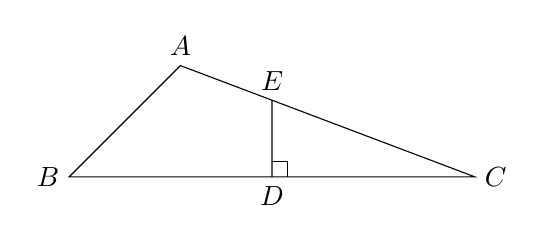
\begin{tikzpicture}
        \draw (0,0) ++ ({-sqrt(2)},0) node [left] {$B$} coordinate (B);
        \draw (0,0) ++ ({sqrt(14)},0) node [right] {$C$} coordinate (C);
        \draw (0,{sqrt(2)}) node [above] {$A$} coordinate (A);
        \draw (A) -- (B) -- (C) -- cycle;
        \path [name path = AC] (A) -- (C);
        \path [name path = perp] ($(B)!0.5!(C)$) node [below] {$D$} coordinate (D) --++ (0,{sqrt(2)});
        \path [name intersections = {of = AC and perp, by = E}];
        \draw (E) node [above] {$E$} -- (D);
        \draw (D) ++ (0,0.2) --++ (0.2,0) --++ (0,-0.2);
    \end{tikzpicture}
\end{center}
\item 设$y=f^{-1}(x)$是函数$f(x)=\dfrac x2+\dfrac{\pi}8\sin x+\dfrac{\pi}8$, $x\in [-\dfrac{\pi }2,\dfrac{\pi }2]$的反函数, 则函数$y=f(x)+f^{-1}(x)$的最小值等于\blank{50}.
\item 函数$f(x)=x$, $g(x)=x^2-x+2$. 若存在$x_1, x_2,\cdots,x_n\in [0,\dfrac 92]$, 使得$f(x_1)+f(x_2)+...+f(x_{n-1})+g(x_n)=g(x_1)+g(x_2)+...+g(x_{n-1})+f(x_n)$, 则$n$的最大值为\blank{50}.
\item 下列函数中既是奇函数, 又在区间$(0,+\infty)$上单调递减的函数为\bracket{20}.
\fourch{$y=\sqrt x$}{$y=\log_{\frac 12}x$}{$y=-x^3$}{$y=x+\dfrac 1x$}
\item 参数方程$\begin{cases} x=3t^2+4,\\ y=t^2-2, \end{cases}$($t$为参数, 且$0\le t\le 3$)所表示的曲线为\bracket{20}.
\fourch{直线}{圆弧}{线段}{双曲线的一支}
\item 将函数$y=\sin (2x-\dfrac{\pi}3)$图像上的点$P(\dfrac{\pi}4,t)$向左平移$s$($s>0$)个单位长度得到点$P'$, 若$P'$位于函数$y=\sin 2x$的图像上, 则\bracket{20}.
\twoch{$t=\dfrac 12$, $s$的最小值为$\dfrac{\pi}6$}{$t=\dfrac{\sqrt 3}2$, $s$的最小值为$\dfrac{\pi}6$}{$t=\dfrac 12$, $s$的最小值为$\dfrac{\pi}3$}{$t=\dfrac{\sqrt 3}2$, $s$的最小值为$\dfrac{\pi}3$}\item 已知以下三个陈述句:\\
$p$: 存在$a\in \mathbf{R}$且$a\ne 0$, 对任意的$x\in \mathbf{R}$, 均有$f(2^{x+a})<f(2^x)+f(a)$恒成立;\\
$q_1$: 函数$y=f(x)$是定义域为$\mathbf{R}$的减函数, 且对任意的$x\in \mathbf{R}$, 都有$f(x)>0$;\\
$q_2$: 函数$y=f(x)$是定义域为$\mathbf{R}$的增函数, 存在$x_0<0$, 使得$f(x_0)=0$;\\
用这三个陈述句组成两个命题, 命题$S$: ``若$q_1$, 则$p$''; 命题$T$: ``若$q_2$, 则$p$''. 关于$S,T$以下说法正确的是\bracket{20}.
\twoch{只有命题$S$是真命题}{只有命题$T$是真命题}{两个命题$S,T$都是真命题}{两个命题$S,T$都不是真命题}
\item 如图, $S$是圆锥的顶点, $O$是底面圆的圆心, $AB$、$CD$是底面圆的两条直径, 且$AB\perp CD$, $SO=4$, $OB=2$, $P$为$SB$的中点.
\begin{center}
    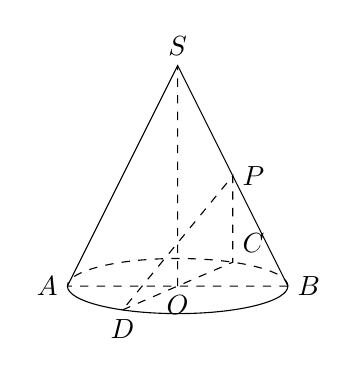
\begin{tikzpicture}[scale = 0.7]
        \draw (-2,0) node [left] {$A$} coordinate (A);
        \draw (2,0) node [right] {$B$} coordinate (B);
        \draw (0,0) node [below] {$O$} coordinate (O);
        \draw (O) ++ (0,4) node [above] {$S$} coordinate (S);
        \draw ($(S)!0.5!(B)$) node [right] {$P$} coordinate (P);
        \draw ({2*cos(-120)},{0.5*sin(-120)}) node [below] {$D$} coordinate (D);
        \draw ({2*cos(60)},{0.5*sin(60)}) node [above right] {$C$} coordinate (C);
        \draw (A) arc (180:360:2 and 0.5) -- (S) -- (A);
        \draw [dashed] (B) arc (0:180:2 and 0.5) -- (B) (D) -- (C) -- (P) -- cycle (O) -- (S);
    \end{tikzpicture}
\end{center}
(1) 求圆锥的体积;\\
(2) 求异面直线$SA$与$PD$所成角的大小(结果用反三角函数值表示).
\item 已知函数$f(x)=\cos x(\sin x+\cos x)-\dfrac 12$.\\
(1) 若$0<\alpha <\dfrac{\pi}2$, 且$\sin \alpha =\dfrac{\sqrt 2}2$, 求$f(\alpha)$的值;\\
(2) 求函数$f(x)$的最小正周期, 及函数$f(x)$在$[0,\dfrac\pi 2]$上的递减区间.
\item 新冠肺炎疫情造成医用防护服紧缺, 某地政府决定为防护服生产企业A公司扩大生产提供$x$($x\in [0,10]$)(万元)的专项补贴, 并以每套$80$元的价格收购其生产的全部防护服. $A$公司在收到政府$x$(万元)补贴后, 防护服产量将增加到$t=k\cdot (6-\dfrac{12}{x+4})$(万套), 其中$k$为工厂工人的复工率($k\in [0.5,1]$). $A$公司生产$t$万件防护服还需投入成本$20+8x+50t$(万元).\\
(1) 将$A$公司生产防护服的利润$y$(万元)表示为补贴$x$(万元)的函数(利润不包含政府补贴);\\
(2) 若对任意的$x\in [0,10]$(万元), $A$公司都不会产生亏损, 求复工率$k$的取值范围.
\item 已知抛物线$y^2=4x$的焦点为$F$, 直线$l$交抛物线于不同的$A$、$B$两点.\\
(1) 若直线$l$的方程为$y=x-1$, 求线段$AB$的长;\\
(2) 若直线$l$经过点$P(-1,0)$, 点$A$关于$x$轴的对称点为$A'$, 求证: $A'$、$F$、$B$三点共线;\\
(3) 若直线$l$经过点$M(8,-4)$, 抛物线上是否存在定点$N$, 使得以线段$AB$为直径的圆恒过点$N$? 若存在, 求出点$N$的坐标, 若不存在, 请说明理由.
\item 无穷数列$\{a_n\}$($n\in \mathbf{N}^*$), 若存在正整数$t$, 使得该数列由$t$个互不相同的实数组成, 且对于任意的正整数$n$, $a_{n+1},a_{n+2},\cdots,a_{n+t}$中至少有一个等于$a_n$, 则称数列$\{a_n\}$具有性质$T$, 集合$P=\{p|p=a_n, \ n\in \mathbf{N}^*\}$.\\
(1) 若$a_n=(-1)^n$, $n\in \mathbf{N}^*$, 判断数列$\{a_n\}$是否具有性质$T$;\\
(2) 数列$\{a_n\}$具有性质$T$, 且$a_1=1$, $a_4=3$, $a_8=2$, $P=\{1,2,3\}$, 求$a_{11}$与$a_{14}$的值;\\
(3) 数列$\{a_n\}$具有性质$T$, 记集合$B=\{m|a_m=a_1, \ m\in \mathbf{N}^*\}$, 将集合$B$中的所有元素按从小到大的顺序排列, 得到数列$\{i_n\}$, 记$b_n=i_{n+1}-i_n$, $n\in \mathbf{N}^*$. 证明: 若数列$\{b_n\}$具有性质$T$, 则数列$\{b_n\}$是常数列.
\end{enumerate}
\end{document}